%!TEX root = ../Combinatorics.tex
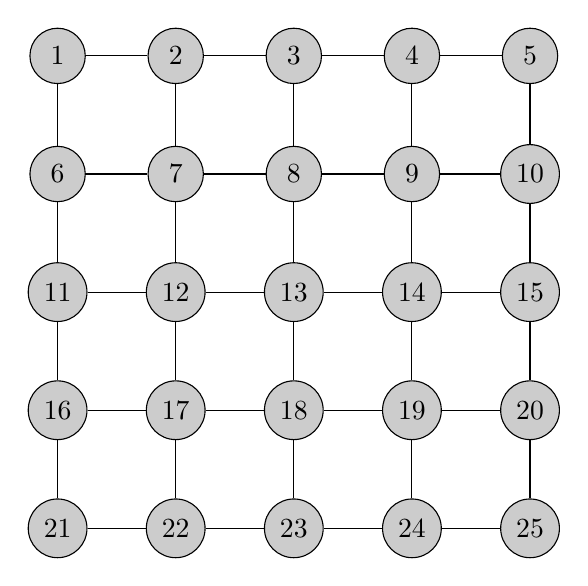
\begin{tikzpicture}[darkstyle/.style={circle,draw,fill=gray!40,minimum size=20}]
  \foreach \x in {0,...,4}
    \foreach \y in {0,...,4} 
       {\pgfmathtruncatemacro{\label}{\x - 5 *  \y +21}
       \node [darkstyle]  (\x\y) at (1.5*\x,1.5*\y) {\label};} 

  \foreach \x in {0,...,4}
    \foreach \y [count=\yi] in {0,...,3}  
      \draw (\x\y)--(\x\yi) (\y\x)--(\yi\x) ;

\end{tikzpicture}
\begin{tikzpicture}[darkstyle/.style={circle,draw,fill=gray!40,minimum size=20}]
%[xscale=.8,yscale=.75]

%\draw  (-3,3) ellipse (2 and 3);
%\draw  (3,3) ellipse (2 and 3);

% %V side
% \def\vx{-1.5}
% \draw  (2.8341+\vx,3.8393) ellipse (1.1649 and 1.3675);
% \node (v2) at (2.6853+\vx+1,5.5201) {$V$};

% \draw (2.4996+\vx,4.0144) node[](v4){\textbullet};
% \draw (2.4996+\vx,4.0144) node [right]  {\footnotesize $v_0$};

% % \draw (2.4996+\vx,4.0144) ellipse (0.7 and 0.7) ;
% % \node(vr1) at (2.4996+\vx,4.0144) {};
% % \node(vr2) at (2.4996+\vx,4.0144+.7) {};
% % \draw  (vr1) edge[<->] node[auto]{\footnotesize $r$}(vr2);

% % \draw (2.4996+\vx,4.0144-.4) node[](v){\textbullet};
% % \draw (2.4996+\vx,4.0144-.4) node [right]  {\footnotesize $v$};

% %U side
% \draw (-3.1,3.6) node (v5) {}ellipse (1.8533 and 2.5917);
% \node (v1) at (-3.3313,6.4532+.3) {$U$};

% \draw[opacity=.5]  (v5) ellipse (1.6 and 1.5);
% \node[opacity=.5] at (-3.0112,1.728) {$\Omega$};

% \draw  (-3.616,3.5459)  node[](v3){\textbullet};
% \draw  (-3.616,3.5459)  node [right]  {\footnotesize $u_0$};

% % \draw   (-3.616,3.5459) ellipse (1 and 1);
% % \node(vCr1) at (-3.616,3.5459)  {};
% % \node(vCr2) at (-3.616,3.5459+1) {};
% % \draw  (vCr1) edge[->,{<->}] node[auto]{\footnotesize $Cr$}(vCr2);

% % \draw (-3.616-.5,3.5459-.4)  node[] (pv){\textbullet};
% % \draw (-3.616-.5,3.5459-.4)  node [right] {\footnotesize $wr+u_0$};

% %Bridge
% \draw  (v3) edge[bend left,<-,dashed, shorten >=-3] node[pos=.65, auto]{$T$}(v4);

\def\slope{.5}

% \foreach \x in {0,...,4}
% 	\foreach \y in {0,...,4} 
%         \node at (1.5*\x,1.5*\y) {};

\node (s1) at (0,0) {};
\node (e1) at (2,1) {};
\draw (s1) edge[->] node[auto] {$x_n$} (e1);


% \draw  (v) edge[bend left,->,dashed, shorten >= 2, shorten <= -3] node[near start, auto]{$T$}(pv);

\end{tikzpicture}